\subsection{Modified Butterfly} \label{subsec:modbutterfly}

\subsubsection*{Allgemein}

Der Modified Butterfly ist eine Erweiterung des klassichen
Butterfly Algorithmus und wurde von Denis Zorin, Peter Schröder und Wim Sweldens entwickelt.
Der Unterteilungsalgorithmus garantiert mit der Modifikation \(C^1\) stetige Flächen
für beliebige Dreiecksnetze.
\cite[S. 72ff]{Zorin.subdivcourse}
\cite{Gamasutra}
\cite{Sharp}

\subsubsection*{Unterteilungs- und Randregeln}

Der Modified Butterfly kann wie auch schon der Butterfly in zwei Schritten zusammengefasst werden:
\begin{enumerate}
\item Berechne für jede Kante einen Edge Point.
\item Ersetze jedes Dreieck durch vier neue Dreiecke.
\end{enumerate}
Der Unterschied liegt darin, dass die Edge Points beim Modified Butterfly
unterschiedlich berechnet wird. Die Berechnung hängt davon ob,
ob die andliegenden Vertices der Kante regulär oder extraordinär sind.

\paragraph*{Edge Point}

\begin{figure}
\centering
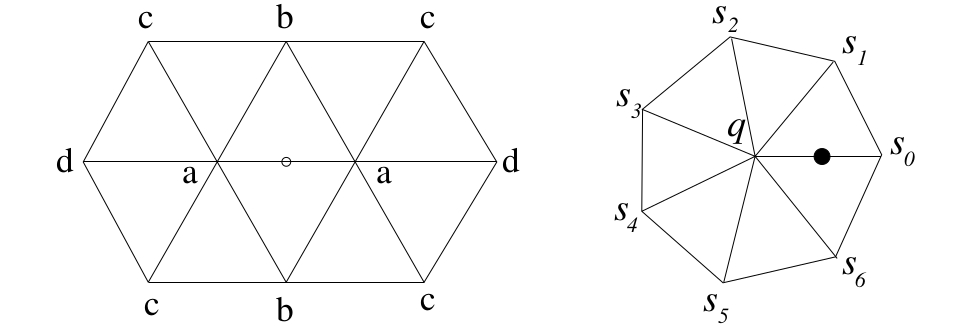
\includegraphics[width=0.8\textwidth]{content/media/sd_modbutterfly_mask.jpg}
\caption{Modified Butterfly Ten-Point Stencil und Maske für einen extraordinären Vertex
\cite{Zorin:1996:ISM:237170.237254}}
\label{fig:sd_modbutterfly_mask}
\end{figure}

Für die Berechnung des Edge Points werden vier Fälle unterschieden:
\begin{description}
\item[Kante verbindet zwei reguläre Vertices \((Valenz = 6)\):]
In diesem Fall wird eine Erweiterung
des Butterfly Schemas verwendet. Das sogenannte Ten-Point Stencil ist in \autoref{fig:sd_modbutterfly_mask} links abgebildet.\\
Die Gewichte sind:
\(a = 1/2 - w,\ b = 1/8 + 2w,\ c = -1/16 - w,\ d = w\).\\
\(w\) kann dabei geeignet klein gewählt werden.
Zorin verwendet in \cite{Zorin:1996:ISM:237170.237254} \(w = 0\).
In diesem Fall ist das Ten-Point Stencil identisch mit dem original
Butterfly Eight-Point Stencil.
\item[Kante verbindet K-Vertex \((Valenz \neq 6)\) und Sechs-Vertex \((Valenz = 6)\):]
In diesem Fall wird das rechte Schema aus \autoref{fig:sd_modbutterfly_mask} verwendet.
Die Gewichte werden abhängig von der Valenz \(K\) verschieden gewählt.\\
\(j = 0, \ldots, K - 1\ und\ q = 3/4\)
\begin{itemize}
 \item \(K = 3\): \(s_0 = 5/12,\ s_{1,2} = -1/12\)
 \item \(K = 4\): \(s_0 = 3/8,\ s_{2} = -1/8,\ s_{1,3} = 0\)
 \item \(K >= 5\): \(s_j = (\frac{1}{4}+ cos(\frac{2 \pi j}{K}) + \frac{1}{2} * cos(\frac{4 \pi j}{K}))/K\)
\end{itemize}
\item[Kante verbindet zwei extraordinäre Vertices:]
Es wird nach dem obigen Schema jeweils für beide Vertices ein Edge Point bestimmt und
davon der Durchschnitt errechnet.
\item[Randkante:] Die Randregel ist mit den Gewichten
\(s_{-1} = -1/16,\ s_0 = 9/16,\ s_1 = 9/16,\ s_2 = -1/16\).
identisch zur Butterfly Randregel
(\autoref{fig:sd_butterfly_mask}).
\end{description}
\cite{Zorin:1996:ISM:237170.237254}
\cite[S. 72ff]{Zorin.subdivcourse}
\cite{Gamasutra}
\cite{Sharp}


\paragraph*{Face Split}
Der Face Split ist identisch mit dem Butterfly Face Split.
\cite{Zorin:1996:ISM:237170.237254}
\cite[S. 72ff]{Zorin.subdivcourse}

\paragraph*{Erweiterte Randregeln}

Für den Modified Butterfly Algorithmus gibt es noch eine ganze Reihe von
Randregeln. Diese treten dann ein, wenn die Maske für die Unterteilung zu groß ist
(ein einzelnes Randdreieck \ldots).
Diese Regeln und Sonderfälle werden jedoch ziemlich komplex und aufwändig in der Implementierung
und sind nicht in Subvis implementiert. Daher werden diese hier nicht weiter diskutiert.
Bei weiterem Interesse ist das Dokument \cite[S. 74f]{Zorin.subdivcourse}
empfehlenswert.
